% !TeX encoding = UTF-8
% !TeX spellcheck = en_GB
% !TeX root = tcas.tex
\documentclass{article}
\usepackage[utf8]{inputenc}
\usepackage{authblk}
\usepackage{setspace}
\usepackage[margin=3cm]{geometry}
\usepackage{graphicx}
\usepackage{subcaption}
\usepackage{amsmath}
\usepackage{amsthm}
\usepackage{biblatex}
\usepackage{amssymb}
\usepackage{cleveref}
\addbibresource{tcas.bib}

\title{\textbf{T.C.A.S.}: \textbf{T}CAS \textbf{C}an \textbf{A}lways \textbf{S}olve \\
		\large Numerical Analysis: a Concrete Computational Approach to Limit Evaluation}
\author{Roberto Alessandro Bertolini}

\date{}

\affil{Liceo Nervi Ferrari - Morbegno}
\onehalfspacing

\theoremstyle{plain}
\newtheorem{thm}{Theorem}

\theoremstyle{definition}
\newtheorem{defn}[thm]{Definition}

\begin{document}
	\maketitle
	
	\begin{abstract}
		Evaluating limits by hand can become a trivial task with a bit of exercise, but a regular computer is generally incapable of proceeding intuitively and needs a reliable algorithm in order to be able to reach consistently the same result. 
		While some purely heuristic or naive approaches might, at first glance, seem good enough, they tend to quickly fall apart in real conditions. TCAS is a portable universal C implementation of the Gruntz Algorithm \cite{gruntz}, which at the present day is the most efficient and reliable way of evaluating limits in the exp-log field of operations.
	\end{abstract}

	\tableofcontents
	
	\newpage	
	
	\section{Introduction}
	
	\subsection{The Limit of a Function}
	
	The limit of the function $ f: \mathbf{R} \rightarrow \mathbf{R} $ is defined as the following:
	
	\begin{defn}
		\[ 
		\lim_{x \to x_{0}}{f(x) = l} 
		 \]
		 
		 If and only if \( 
		 \forall \varepsilon > 0 \enspace \exists \enspace \delta(\varepsilon) \mid \forall x \in D_{f}, 0 < \mid x - x_{0} \mid < \delta \implies \mid f(x) - l \mid < \varepsilon, where x_{0}, \varepsilon \in \mathbf{R}
		  \)
	\end{defn}
	
	\subsection{Polish Notation}
	
	Jan Lukasiewicz devised the so-called Polish notation \cite{wiki:polish} in 1924; it is a prefix notation, where the operator precedes its operands.
	As long as the number of operands is defined as constant, there can't be an ambiguity in the order of evaluation, so this notation doesn't strictly require parenthesis.
	Consider the following expression written without parenthesis:
	
	\[
	    8 \times 4 + 3 \times  2 - 6
	\]
	
	Depending on where the parenthesis are placed, it can evaluate to different results:
	
	\[
	    (8 \times 4 + 3) \times (2 - 6) = -140; \quad (8 \times (4 + 3) \times 2) - 6 = 106 
	\]
	
	Now consider a similar expression written using polish notation:
	
	\[
	    \times \times 8 + 4 \enspace 3 - 2 \enspace 6 = -224
	\]
	
	It necessary evaluates to a single result.
	This makes parsing the expression into an abstract syntax tree much easier, as the Parser doesn't have to make educated choices about its interpretation.
	
	\subsection{The Shortcomings of the Naive Approach}
	
	Evaluating a limit might seem easy for a computer, as it should be able to continuously approximate the result with a smaller $\varepsilon$ until the rounding error is acceptable enough, but can this always work?
	Consider the following function:
	
	\[
	    f : y = \frac{1}{x^{\ln{\ln{\ln{\ln{\frac{1}{x}}}}}-1}} \tag{1.3} \label{eq:toinfinity}
	\]
	
	Its graph is the following: \cref{fig:limoff1}, where it seems that for values of x closer to zero the function tends to zero, yet if we compute the limit: \(\lim{x \to 0^{+}}{f(x) = +\infty}\), so the function should have a vertical asymptote in zero. We just can't see it in the graph because it becomes visible for \(x \approx 4.29 \times 10 ^{-1656521}\). A computer trying to approximate the result would have stopped long before this value, returning zero.
	
	What if we try instead to recursively apply L'Hôpital's rule \cite{wiki:hopital} until we reach a clear result?
	Consider the following functions:
	
	\[
	    f(x) = e^{x} + e^{-x}
	    \] 
	    \[
	    g(x) = e^{x} - e^{-x}
    \]
    
    \[
        \lim_{x \to \infty}{\frac{f(x)}{g(x)}} = \lim_{x \to \infty}{\frac{f''(x)}{g''(x)}} = \lim_{x \to \infty}{\frac{e^{x} + e^{-x}}{e^{x} - e^{-x}}}
    \]
	
	So recursively applying L'Hôpital's rule would not work in this case.
	
	\section{The Gruntz Algorithm}
	
	\subsection{The Most Rapidly Varying Subexpressions}
	
	The MRV set of an expression is defined as the following:
	
	\begin{defn}
	    \[
	    mrv(f(x)) = \begin{cases}
	    	\{\} \quad if \enspace x \ntriangleleft f(x) \\
	    	\{g(x) \mid g(x) \ntriangleleft f(x) \wedge (\nexists \enspace h(x) \ntriangleleft f(x) \mid h(x) \succ g(x)))\}
	    \end{cases}
    	\]
	\end{defn}
	
	\subsection{Power Series Representation}
	
	\subsection{Caveats and Limitations}
	
	\section{T.C.A.S.}
	
	\subsection{Expression Parsing}
	
	\subsection{Finding the MRV}
	
	\subsection{Evaluating the Result}
	
	\subsection{Performance Considerations}
	
	\printbibliography
	
	\newpage
	\appendix
	\begin{figure}
	    \centering
	    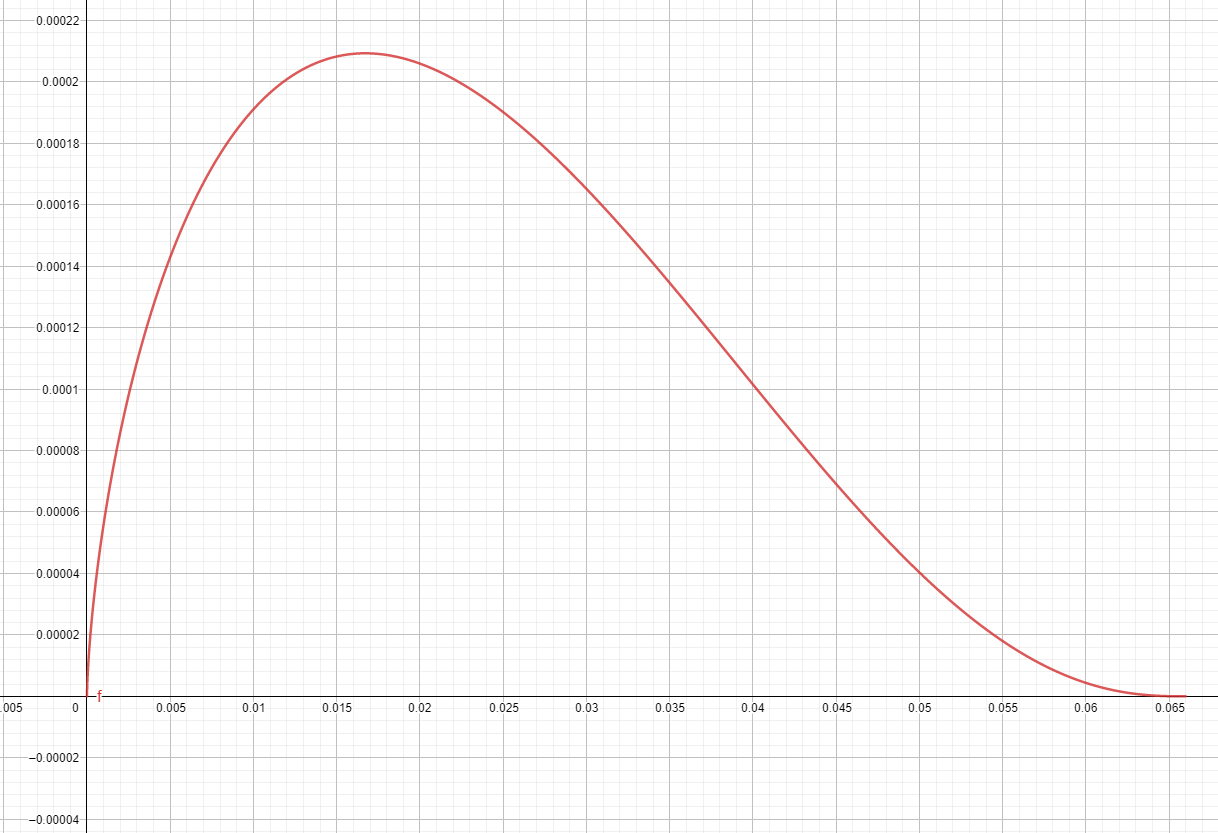
\includegraphics[width=0.7\textwidth]{img/limoff1.PNG}
	    \caption{The graph of the function \eqref{eq:toinfinity}}\label{fig:limoff1}
	\end{figure}
	
\end{document}
